\section{Introduction}
\label{sec:intro}

Research produces a rich, branching knowledge object: months of hypotheses tested and rejected, implementation tricks discovered through trial and error, design alternatives weighed against each other, and the full exploration trajectory that explains why the final approach was chosen.
Publishing compiles this object into a linear narrative~\citep{medawar1963fraud, canini2026stopwriting}, discarding failed experiments, tacit engineering knowledge, and the branching process to satisfy the conventions of human-readable storytelling~\citep{rosenthal1979filedrawer, franco2014publication}.
This compilation cost, a consequence of the documentation convention rather than any particular file format, was tolerable when every consumer of a paper was human.
It is not when AI agents routinely read papers to understand a field, reproduce experiments to validate findings, and extend published methods to new settings~\citep{lu2024aiscientist, liu2026ainative}: each task requires precisely the knowledge that compilation discards (Figure~\ref{fig:overview}).
More specifically, the compilation incurs two structural costs.

\begin{figure}[t]
    \centering
    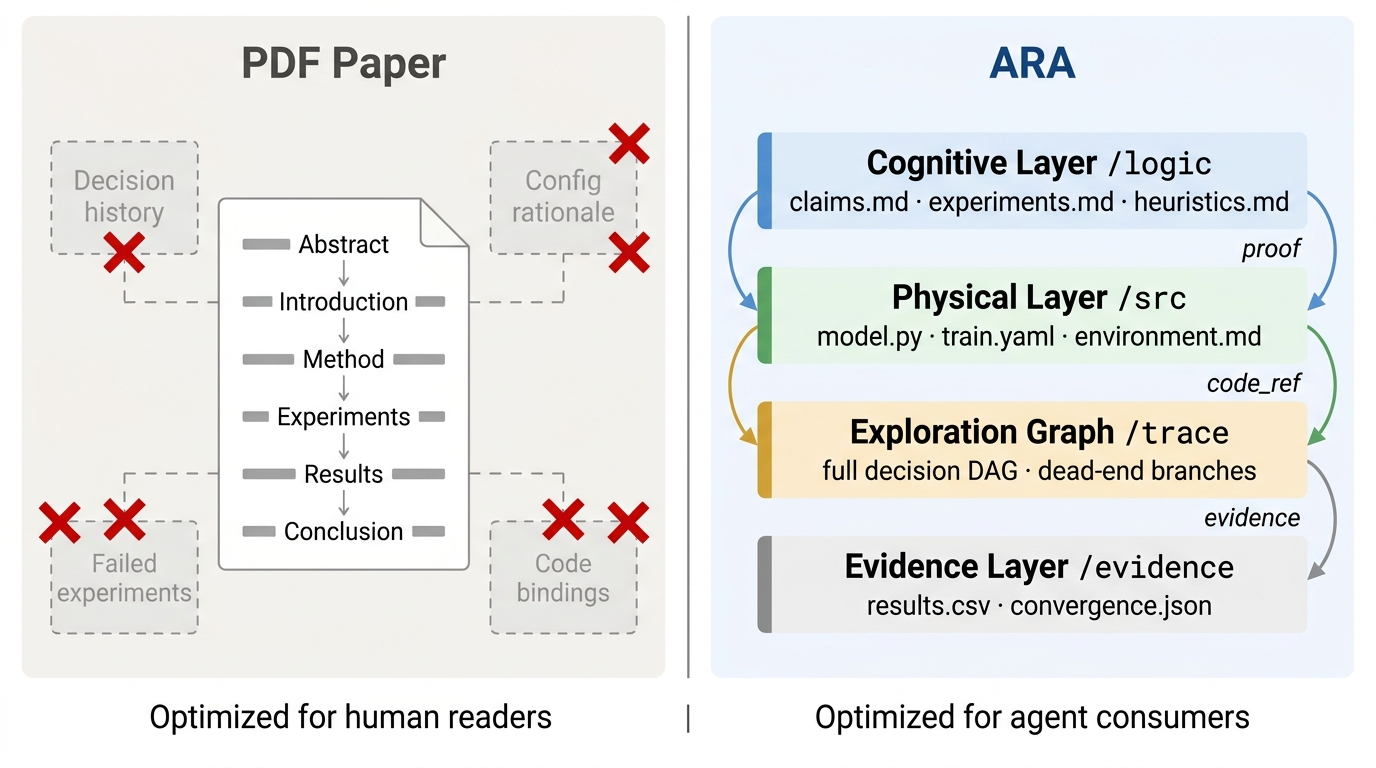
\includegraphics[width=\linewidth]{figures/fig_legacy_vs_ara_v6.png}
    \caption{Publishing compiles a rich research object into a lossy narrative (left); \ara{} preserves the original as a high-fidelity, agent-executable knowledge package (right).}
    \label{fig:overview}
\end{figure}
The first is the \textbf{Storytelling Tax}: the systematic erasure of research process knowledge imposed by compilation into narrative (Figure~\ref{fig:storytelling-tax}).
Research does not proceed linearly---it branches, backtracks, and accumulates hard-won failure knowledge before converging on a publishable result~\citep{kuhn1962structure,medawar1963fraud}.
Narrative compilation flattens this process into a polished linear story, discarding every failed experiment, rejected hypothesis, and abandoned approach.
This emphasis on success leaves failures undocumented; although modern platforms archive final artifacts, the branching research process remains unrecorded, causing independent rediscovery of the same dead ends across groups~\citep{rosenthal1979filedrawer, franco2014publication}.
Our own analysis of the METR eval-analysis-public dataset~\citep{wijk2025rebench}, covering 24{,}008 agent runs across 21 frontier models on RE-Bench, quantifies the cost (per-task breakdown in Appendix~\ref{app:exploration-tax}): failed runs account for \textbf{90.2\%} of total dollar cost (and 59.2\% of tokens), with a median failed-to-success token ratio of \textbf{113$\times$}, agents without access to prior failure records must independently rediscover every dead end.
Equally lost is the record of human \emph{judgment} along the trajectory: every rejection, revision, and endorsement is a preference signal over what constitutes good research, the scarce resource that binds once agents shoulder the grunt work. Narrative compilation discards this signal; a preserved trajectory renders it as structured supervision that compounds across projects.

The second is the \textbf{Engineering Tax}: the gap between \emph{reviewer-sufficient} and \emph{agent-sufficient} documentation (Figure~\ref{fig:info-gap}).
The paper communicates its contribution at the level of detail needed to convince a human reviewer; the codebase provides an implementation but not the operational specification needed to execute it.
Between the two lies tacit knowledge~\citep{polanyi1966tacit}---algorithmic tricks, implementation decisions, and configuration choices---knowledge that exists in no written document and is transmitted only through direct lab contact or painstaking reverse-engineering.
We quantify this void by classifying each of PaperBench's 8{,}921 expert-annotated reproduction requirements across 23 ICML~2024 papers~\citep{starace2025paperbench} against its source PDF (per-category breakdown and gap-type taxonomy in Appendix~\ref{app:gap-types}): despite widespread artifact sharing, only \textbf{45.4\%} are fully specified.
Code development is the most underspecified category (37.3\% sufficient), and missing hyperparameters alone account for 26.2\% of all gaps (full breakdown in Appendix~\ref{app:gap-types}): a fundamental mismatch between the precision at which papers are written (sufficient to produce belief) and the precision at which agents must operate (sufficient to produce correct execution)~\citep{stodden2016enhancing, baker2016reproducibility}.

Both taxes have persisted throughout the history of research because the human reader has always been the bandwidth-limited layer processing a vast, non-linear research trajectory.
Capable AI agents now offer a more efficient, human-proximal proxy that processes the trajectory at machine bandwidth on the reader's behalf, and three trends suggest what such an artifact should look like.
\textbf{First}, AI agents have become indispensable research companions, co-authoring code, running experiments, and iterating on hypotheses alongside humans~\citep{lu2024aiscientist}, with LLM adoption associated with paper-production increases of 23.7\%--89.3\% across scientific fields~\citep{kusumegi2025scientific}; the full research trajectory (every failure, implementation trick, configuration choice, design pivot) is now captured as machine-readable text in researcher-agent sessions, yet no protocol preserves it as a first-class output.
\textbf{Second}, humans and AI agents have divergent information needs: humans skim abstracts and figures~\citep{renear2009strategic}, while agents benefit from exhaustive detail that strictly improves reproduction, verification, and extension, so a single artifact optimized for human narrative can no longer serve both.
\textbf{Third}, research is scaling into a massively parallel enterprise where agents fork, extend, and merge each other's work at machine speed, shifting the bottleneck from individual productivity to artifact \emph{operability}: narrative PDFs, compiled for sequential human reading, cannot be forked, diffed, or merged, but a structured, lossless artifact can, letting research compound like software.

\begin{figure}[t]
    \centering
    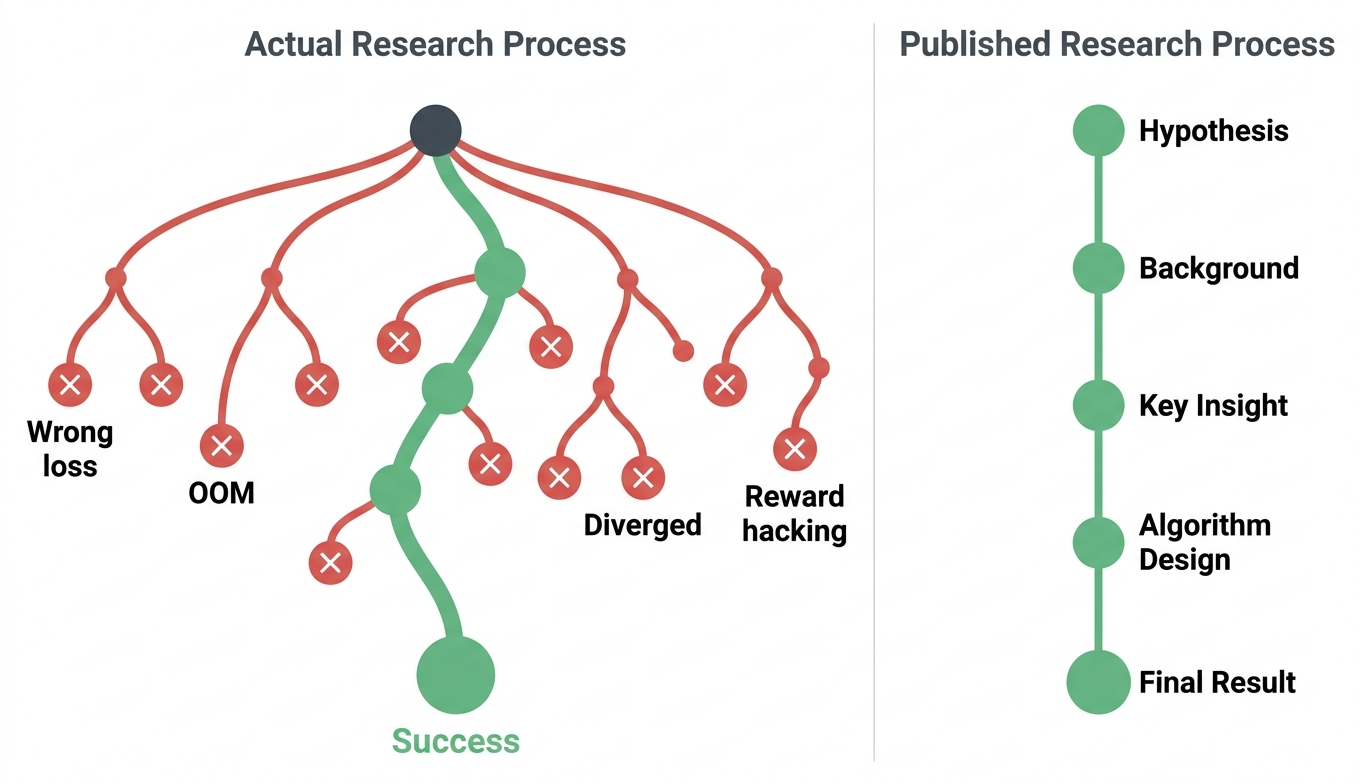
\includegraphics[width=0.95\linewidth]{figures/fig_exploration_tax.png}
    \caption{The Storytelling Tax: research proceeds as a branching tree with dead ends (left), but publication compiles it into a linear narrative (right), discarding all failure knowledge.}
    \label{fig:storytelling-tax}
\end{figure}
    
Existing efforts address fragments of this problem.
The FAIR principles~\citep{wilkinson2016fair} mandate findable, accessible data but say nothing about the structure of research \emph{arguments}.
RO-Crate~\citep{soilandreyes2022rocrate} packages research artifacts as archival bundles, not executable objects.
Nanopublications~\citep{groth2010nanopub} formalize atomic claims but lack the execution layer needed for reproduction.
The emerging \texttt{AGENTS.md} standard~\citep{openai2025agentsmd} provides agent-oriented documentation for code repositories but does not address the epistemic structure of research itself.
None of these efforts jointly structure scientific logic, executable code, and exploration history into a single operable object (\S\ref{sec:related}).

We propose the \textbf{Agent-Native Research Artifact (\ara{})}, a protocol that recasts the primary research object from narrative document to agent-executable knowledge package, with papers serving as compiled views of the underlying artifact (Figure~\ref{fig:overview}).
\ara{} organizes research into four interlocking layers: \emph{structured scientific logic} that distills the paper's conceptual abstractions into queryable claims and dependency graphs; \emph{executable code} with full operational specifications; an \emph{exploration graph} preserving the branching research process---failed experiments, rejected hypotheses, and design pivots---that narrative compilation discards; and \emph{grounded evidence} binding every claim to its raw empirical outputs.
Instead of parsing prose, reverse-engineering repositories, and rediscovering dead ends, an agent operating on an \ara{} artifact can query structured claims, execute declarative specifications, and build on the full decision history directly---a research object designed not to be read, but to be \emph{operated}.

To build the ecosystem around \ara{}, we develop three enabling mechanisms.
The \textbf{Live Research Manager} (\S\ref{sec:live-pm}) captures research decisions and dead ends as natural side-effects of everyday development, producing conforming artifacts without additional documentation burden.
The \textbf{\ara{} Compiler} (\S\ref{sec:ingestor}) translates legacy PDFs, repositories, and supplementary materials into \ara{} format, providing backward compatibility with the existing publication ecosystem.
The \textbf{\ara{}-Native Review System} (\S\ref{sec:review-system}) automates structural verification and budget-aware reproduction (analogous to a grammar checker for prose), redirecting expert attention from mechanical checking to judgment---significance, novelty, and taste~\citep{aczel2021billiondollar}.

\begin{figure}[t]
    \centering
    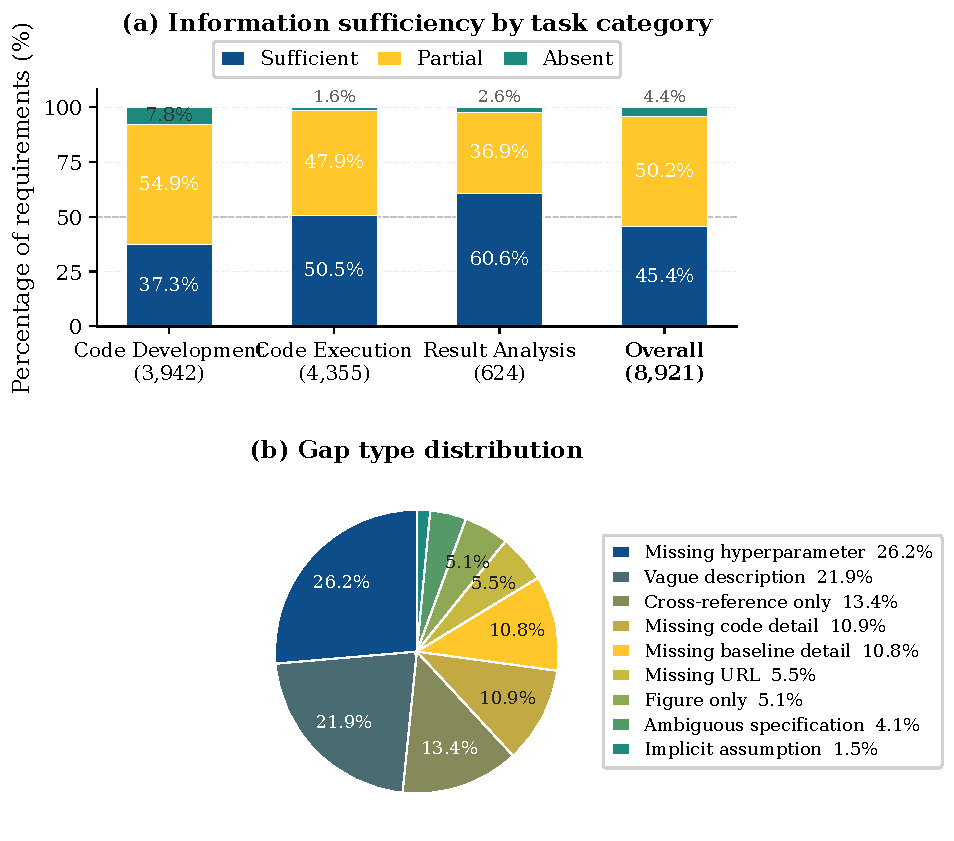
\includegraphics[width=\linewidth]{figures/fig_info_gap.pdf}
    \caption{The reproduction information gap across 8,921 PaperBench requirements. \textbf{(a)}~PDFs systematically under-specify code development tasks. \textbf{(b)}~The three largest gap types are precisely the categories \ara{}'s structured layers address.}
    \label{fig:info-gap}
\end{figure}
\paragraph{Contributions.}
\begin{itemize}[leftmargin=*, itemsep=2pt]
    \item We identify two structural costs of compiling research into narrative---the \textbf{Storytelling Tax} and the \textbf{Engineering Tax}---and introduce the \textbf{Agent-Native Research Artifact (\ara{})}: a protocol that recasts the primary research object from narrative document to agent-executable knowledge package organized into four interlocking layers (\S\ref{sec:protocol}).
    \item We develop three enabling mechanisms: a \textbf{Live Research Manager} (\S\ref{sec:live-pm}) that captures research decisions during ordinary development; an \textbf{\ara{} Compiler} (\S\ref{sec:ingestor}) that translates legacy PDFs and repositories into \ara{} format; and an \textbf{\ara{}-Native Review System} (\S\ref{sec:review-system}) that automates objective verification (analogous to a grammar checker for prose) so human reviewers can focus on judgment.
    \item We evaluate \ara{} across three layers of research utility (\S\ref{sec:eval}): \emph{understanding} (what an agent can extract from the artifact), \emph{reproduction} (whether the agent can re-execute the paper's experiments), and \emph{extension} (whether the agent can build beyond the documented results and discover genuinely new findings, the defining goal of research). Across all three layers, agents operating on an \ara{} consistently outperform those reading the paper PDF and its associated code repository.
\end{itemize}
